\documentclass{article}
\usepackage[utf8]{inputenc}
\usepackage{amsmath, amssymb, amsthm, cancel}
\usepackage{enumitem}
\usepackage{caption}
\usepackage{graphicx}
\usepackage[top=1in, bottom=1in, left=1in, right=1in]{geometry}
\usepackage{float}
\usepackage{booktabs}
\usepackage{array}
\usepackage{multirow}

\title{\textbf{CSCI4150U: Data Mining}\\K-Means and Hierarchical Clustering}
\author{Syed Naqvi \\ Student ID: 100590852}
\date{\today}

\begin{document}

\maketitle

\begin{abstract}
blablabla
\end{abstract}

\section{Introduction}

\subsection{Methodology}
Datasets used in this analysis are sourced from the \textit{UC Irvine Machine Learning Repository} and include:
\begin{itemize}
    \item \textbf{Breast Cancer Wisconsin (Diagnostic)}
    \item \textbf{Waveform Database Generator (Version 1)}
\end{itemize}

We evaluate the following clustering algorithms:
\begin{itemize}
    \item \textbf{K-means Clustering}
    \item \textbf{Hierarchical Clustering} (Single Link, Complete Link, and Group Average)
\end{itemize}

For K-means clustering, model \( k \) values range from 1 to 6 for the \textit{Breast Cancer Wisconsin (Diagnostic)} dataset
and 2 to 6 for the \textit{Waveform Database Generator (Version 1)} dataset. Clustering performance is assessed using the Sum of Squared Errors
(SSE) with Euclidean distance as the metric.

\newpage

\subsection{Preprocessing}
To perform accurate clustering, we analyze feature ranges to determine the dataset most needing of standardization.
\begin{figure}[H]
    \centering
    \begin{minipage}[b]{0.49\textwidth}
        \centering
        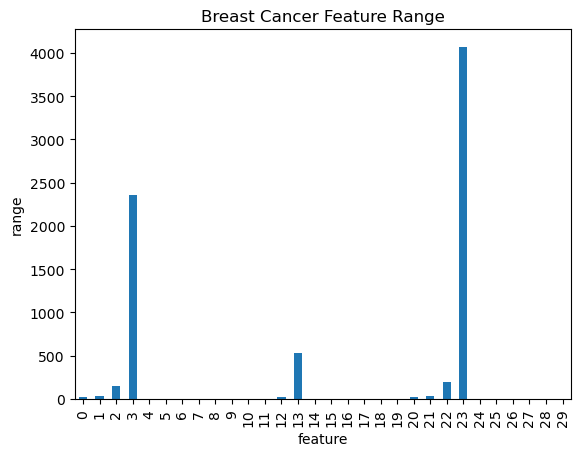
\includegraphics[width=\textwidth]{p_i.png}
        \caption{Pre-Standardized Feature Ranges (Breast Cancer Data)}
    \end{minipage}
    \hfill
    \begin{minipage}[b]{0.49\textwidth}
        \centering
        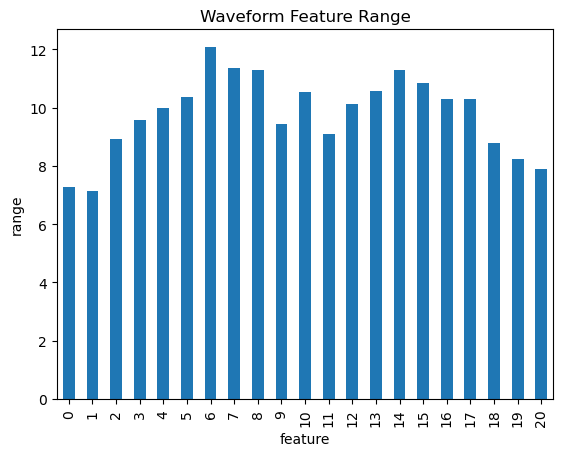
\includegraphics[width=\textwidth]{p_ii.png}
        \caption{Pre-Standardized Feature Ranges (Waveform Data)}
    \end{minipage}
\end{figure}
\begin{figure}[H]
    \centering
    \begin{minipage}[b]{0.49\textwidth}
        \centering
        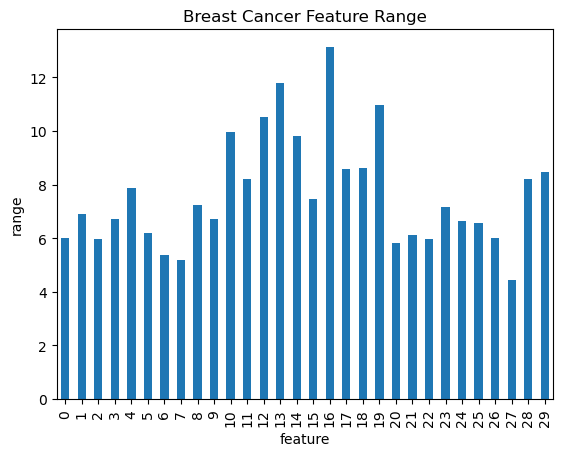
\includegraphics[width=\textwidth]{p_iii.png}
        \caption{Post-Standardized Feature Ranges (Breast Cancer Data)}
    \end{minipage}
    \hfill
    \begin{minipage}[b]{0.49\textwidth}
        \centering
        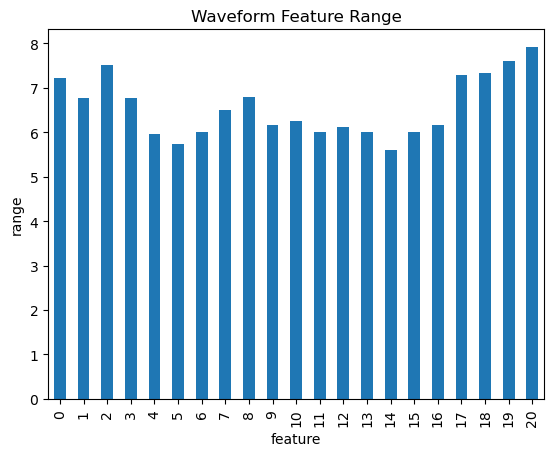
\includegraphics[width=\textwidth]{p_iv.png}
        \caption{Post-Standardized Feature Ranges (Waveform Data)}
    \end{minipage}
\end{figure}

The feature values have now been scaled and are significantly better suitable for clustering. 

\newpage

\section{Part I: K-Means Clustering}
\subsection{Model Selection}
\begin{figure}[H]
    \centering
    \begin{minipage}[b]{0.49\textwidth}
        \centering
        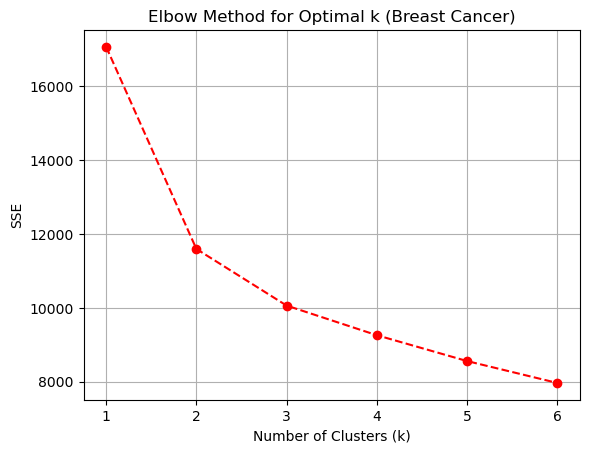
\includegraphics[width=\textwidth]{elbow_cancer.png}
        \caption{Elbow method for selecting optimal K-value (Breast Cancer Dataset)}
    \end{minipage}
    \hfill
    \begin{minipage}[b]{0.49\textwidth}
        \centering
        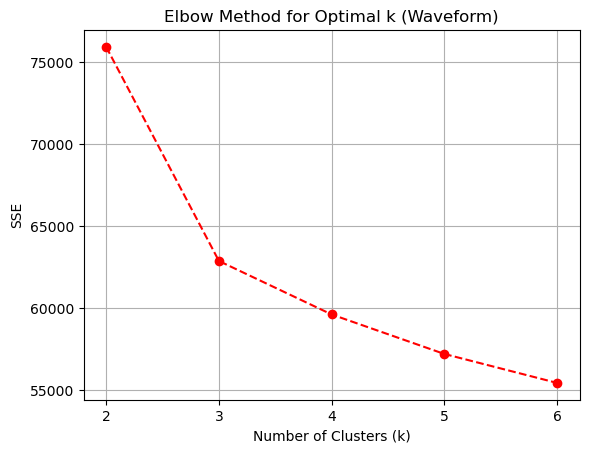
\includegraphics[width=\textwidth]{elbow_waveform.png}
        \caption{Elbow method for selecting optimal K-value (Waveform Dataset)}
    \end{minipage}
\end{figure}

From the above figures, the ideal number of clusters is \textbf{k=2} for the Breast Cancer dataset and \textbf{k=3} for the Waveform dataset. This
suggests there are likely 3 distinct waveforms in the Waveform dataset and two distinct tumor categorizations (malignant or benign)
in the Breast Cancer dataset which is of course consistent with the actual number of unique labels in both datasets.  


\subsubsection{IBk Classification}
Table~\ref{tab:ibk-results} presents the accuracy of IBk classification for K values 1, 3, and 5 across the three datasets.

\begin{table}[H]
    \centering
    \caption{Accuracy of IBk Classification}
    \label{tab:ibk-results}
    \begin{tabular}{|c|c|c|c|}
        \hline
        \textbf{Dataset} & \textbf{K=1} & \textbf{K=3} & \textbf{K=5} \\
        \hline
        letter & 96.03 & 95.62 & 95.52 \\
        \hline
        segment & 97.14 & 96.02 & 95.06 \\
        \hline
        waveform-5000 & 73.62 & 77.7 & 78.94 \\
        \hline
    \end{tabular}
\end{table}

\subsubsection{J48 and AdaBoostM1 Classification}
Table~\ref{tab:j48-adaboost-results} summarizes the accuracy results for J48 with M values of 2 and 4, and AdaBoostM1 with J48 (M=2) as the base classifier.

\begin{table}[H]
    \centering
    \caption{Accuracy of J48 and AdaBoostM1 Classification}
    \label{tab:j48-adaboost-results}
    \begin{tabular}{|c|c|c|c|}
        \hline
        \textbf{Dataset} & \textbf{J48 (M=2)} & \textbf{J48 (M=4)} & \textbf{AdaBoostM1+J48 (M=2)} \\
        \hline
        letter & 87.98 & 86.56 & 95.54 \\
        \hline
        segment & 96.93 & 96.06 & 98.53\\
        \hline
        waveform-5000 & 75.08 & 75.82 & 80.68 \\
        \hline
    \end{tabular}
\end{table}

\subsubsection{NaiveBayes Classification}
Table~\ref{tab:naivebayes-results} provides the accuracy results for NaiveBayes classification on each dataset.

\begin{table}[H]
    \centering
    \caption{Accuracy of NaiveBayes Classification}
    \label{tab:naivebayes-results}
    \begin{tabular}{|c|c|}
        \hline
        \textbf{Dataset} & \textbf{Accuracy (\%)} \\
        \hline
        letter & 64.12 \\
        \hline
        segment & 80.22 \\
        \hline
        waveform-5000 & 80.00 \\
        \hline
    \end{tabular}
\end{table}

\newpage

\section{Part II: Clustering Task}

\subsection{Methodology}
For the clustering task, we use SimpleKMeans to cluster each dataset with specified K values. We use the training set and evaluate each K-means model by measuring the Sum of Squared Errors (SSE). The chosen K values for each dataset are:
\begin{itemize}
    \item \textbf{letter}: K = 11, 24, 38
    \item \textbf{segment}: K = 3, 5, 10
    \item \textbf{waveform-5000}: K = 2, 3, 5
\end{itemize}

\subsection{Results}
Table~\ref{tab:kmeans-sse-results} shows the SSE results for SimpleKMeans clustering for each dataset with different K values.

\begin{table}[H]
    \centering
    \caption{SSE of SimpleKMeans Clustering}
    \label{tab:kmeans-sse-results}
    \begin{tabular}{|c|c|c|c|}
        \hline
        \textbf{Dataset} & \textbf{K=K1} & \textbf{K=K2} & \textbf{K=K3} \\
        \hline
        letter & 16513.56 & 9824.97 & 5132.69 \\
        \hline
        segment & 2173.14 & 1296.73 & 759.97 \\
        \hline
        waveform-5000 & 5465.74 &3846.65 & 3432.81 \\
        \hline
    \end{tabular}
\end{table}

\section{Conclusion}
This report evaluates classification and clustering methods on three datasets using WEKA. IBk, J48, AdaBoostM1, and NaiveBayes are
tested for classification, with AdaBoostM1 using J48 decision trees being the most accurate model across all datasets. SimpleKMeans clustering
SSE is analyzed for different K values where the lowest error values are associated with the highest k values for each dataset.

\end{document}
